\documentclass[11pt]{article}
\usepackage{graphicx}
\usepackage{hyperref}
\usepackage[dvipsnames, svgnames, x11names, hyperref]{xcolor}
\hypersetup{
	colorlinks,
	citecolor=Violet,
	linkcolor=Red,
	urlcolor=Blue}
\usepackage{natbib}
\usepackage{commath, amsmath}
\usepackage{siunitx}
\usepackage{gensymb}

\setlength{\textwidth}{6.5in}
\setlength{\headheight}{0in}
\setlength{\textheight}{8.0in}
\setlength{\hoffset}{0in}
\setlength{\voffset}{0in}
\setlength{\oddsidemargin}{0in}
\setlength{\evensidemargin}{0in}


\title{Homework 10 Solution}

\author{Nana Ama Nyamekye Darpaah}

\begin{document}
	
	\maketitle
	This is my GitHub link: \href{https://github.com/nnd2016/phys-ga2000.git}{Nana Ama's GitHub Link}
	
	
	\section{Introduction}
	In one-dimension(1D), the Schrodinger equation of a particle is expressed as
	
	\begin{equation}
	 -\frac{\hbar^{2}}{2M}\frac{\partial^{2}\psi}{\partial{x}^{2}} = i\hbar\frac{\partial\psi}{\partial t}
	 \label{eq1}
	\end{equation}

	This particle, an electron, was then placed in a box with impenetrable walls in one dimension was solved in questions one and two using the Crank-Nicolson method and the spectral method. Boundary conditions of $\psi(x=0) = \psi(x=L) = 0$ were applied in both cases. The mass of the electron is $M = 9.109 \times 10^{-31} kg$, in abox of length $L = 1 \times 10^{-8} m$. At time $t = 0$, the wavefunction of the electron is of the form 
	\begin{equation}
		\psi(x, 0) = \exp[-\frac{(x-x_{0})^{2}}{2 \sigma^{2}}] \exp(ikx)
		\label{eq2}
	\end{equation}
	where $x_{0} = \frac{L}{2}, \sigma = 1 \times 10^{-10} m$, and $k = 5 \times 10^{10} m^{-1}$
	
	
	\section{Crank-Nicolson Method}
	The Crank-Nicolson equations can be written in the form 
	
	\begin{equation}
		A \psi(t + h) = B \psi(t)
		\label{eq3}
	\end{equation}
with
	\begin{equation}
		\psi(t) = \begin{pmatrix}
			\psi(a, t)\\\psi(2a, t)\\\psi(3a, t)\\ \vdots
		\end{pmatrix}	
	\label{eq4}
	\end{equation}

where $a$ is the spacing of the spacial grid points and $h$ is the size of the time step and the matrices A and B are tridiagonal matrices
   \begin{equation}
   	A = \begin{pmatrix}
   		a_{1} & a_{2}\\
   		 a_{2} & a_{1} & a_{2}&  \\
   		 & a_{2} & a_{1} & a_{2} & \\
   		 & & a_{2} & a_{1} & &\\
   		 & & & \ddots
   	\end{pmatrix}, 
   B = \begin{pmatrix}
   	b_{1} & b_{2}\\
   	b_{2} & b_{1} & b_{2}&  \\
   	& b_{2} & b_{1} & b_{2} & \\
   	& & b_{2} & b_{1} & &\\
   	& & & \ddots
   \end{pmatrix}
\label{eq5}
   \end{equation}
  and 
  \begin{equation}
  	a_{1} = 1 + h\frac{i\hbar}{2ma^{2}} , a_{2} -h\frac{i\hbar}{4ma^{2}}, b_{1} = 1-h\frac{i\hbar}{2ma^{2}}, b_{2} =h\frac{i\hbar}{4ma^{2}} 
  	\label{eq6}
  \end{equation}
	The vector $\psi(t)$ was calculated using the initial wavefunction above numerically by
	\begin{equation}
		v = B\psi
		\label{eq7}
	\end{equation}
	
	 with $N = 1000$ spatial slices and $a = L/N$ for a single step.
	
	where 
	\begin{equation}
		v_{i} = b_{1}\psi_{i} + b_{2}(\psi_{i + 1} + \psi_{i-1})
		\label{eq8}
	\end{equation}

	For the next step, the scipy.banded module was used to solve the linear system $A x = v$, which gives the updated $\psi$ 
	It was then extended to perform repeated steps at a separation $h = 1 \times 10^{-18} s$ .
    An animation of the solution was made at each time step.
	
	\section{Spectral Method}
	Th spectral method involves using a Fourier transform to solve for the k components. With the same 1D Schrodinger equation as in Equation ..., the potential solution to this equation is 
	\begin{equation}
		\psi_{k} =  \sin (\frac{\pi k x}{L} \exp(\frac{iEt}{\hbar}))
		\label{eq9}
	\end{equation}
	with 
	\begin{equation}
		E = \frac{\pi^{2} \hbar^{2} k^{2}}{2ML^{2}}
		\label{eq10}
	\end{equation}
	with a full solution expressed as a linear combination of these individual solutions on grid points $x_{n} = \frac{nL}{N}$
	\begin{equation}
		\psi(x_{n}, t) = \frac{1}{N} \sum_{k = 1}^{N-1} \sin(\frac{\pi k n}{N}) \exp(i\frac{\pi^{2} \hbar k^{2}}{2ML^{2}})
		\label{eq11}
	\end{equation}
	and $b_{k} = \alpha_{k} + i\eta_{k}$ with $\alpha_{k}$ being the real part and $\eta_{k}$, the imaginary part.
	
	A programme was made to calculate these $b_{k}$ coeffficients with the same parameters as those in the Crank-Nicolson method. Discrete sine transformations were performed on each initial wavefunction real and imaginary array at each grid point for all $k=1, \cdots, N-1$.
	The real part of the wavefunction was taken and extended at an arbitrary time using the inverse discrete sine transformation. This programme was tested by making a graph of the wavefunction at time $t = 10^{-16} s$ as seen in Figure ...  The programme was also extended to make an animation. 
	
	
	 
	\section{Discussion of Results}
	These 2 methods produced the same results.
		 
	\begin{figure}[!h]\begin{center} 
			\vspace{12pt}
			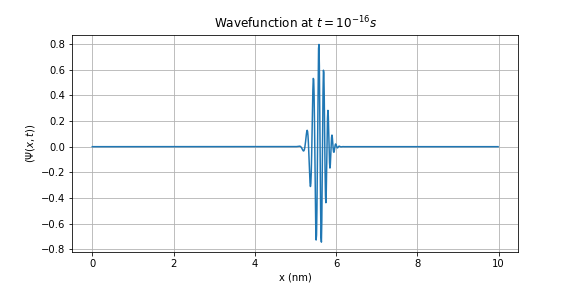
\includegraphics[width=0.7\textwidth]{spectral_test_time.png}
			\caption{Waveform at $ t = 1 \times 10^{-16} s $}
			\label{fig:spectral_test} 
		\end{center}
	\end{figure} 


	\begin{figure}[!h]\begin{center} 
			\vspace{12pt}
			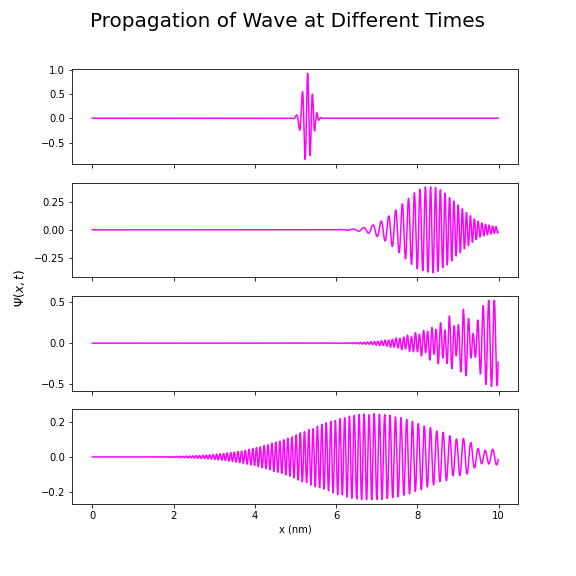
\includegraphics[width=0.7\textwidth]{cn_wave.png}
			\caption{Crank-Nicolson Method}
			\label{fig:cn} 
		\end{center}
	\end{figure} 

	
	 The test at time $t = 1 \times 10^{-16} s$ yielded the plot in Figures  \ref{fig:spectral_test}  The progress of  propagation of the wave can be seen in Figure \ref{fig:cn} where it loses energy as it travels along the positive x direction and meets a boundary (that is the potential barrier), bounces back and travels along the negative x direction effectively changing its waveform. 
	
	
	
	
\end{document}